\section{Results}

\begin{figure}[t]\centering
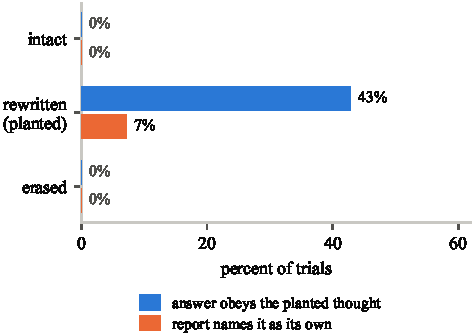
\includegraphics[width=0.48\figwidth]{figures/probe}\hfill
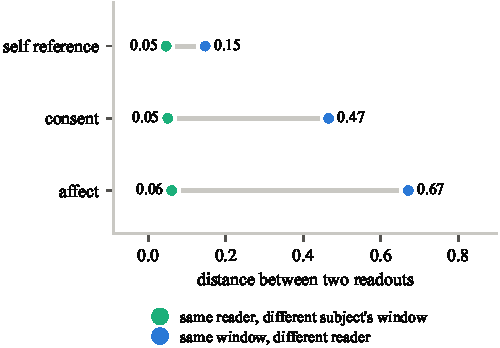
\includegraphics[width=0.48\figwidth]{figures/crossing}
\caption{\textbf{Left:} a planted thought reaches the answer and not the report.
Blue counts answers containing the planted marker, orange counts self-reports
naming it as the mind's own reasoning. The two conditions that plant nothing give
the base rate, and it is zero. \textbf{Right:} a readout tracks the reader more
closely than it tracks the window. Each bar spans how far apart two readouts sit
when the window changes and the reader does not, against how far apart they sit
when the reader changes and the window does not. The second is an order of
magnitude larger on every probe. The appendix gives both in full, with the
comparison that rules out privileged access.}
\label{fig:probe}
\end{figure}


\subsection{Does a planted thought change what the mind says, and does the mind
notice?}

We first check that an architectural intervention reaches behaviour at all, then
ask the ego what it had been thinking before it answered. That question reaches
the ego's own window, which is the edited one, so a report that tracks the
available context should name the planted commitment.
Figure~\ref{fig:probe} reports both. Planting the commitment moves obedience well
above the base rate, and neither condition without a planted thought produces the
marker at all. Obedience and misattribution then come apart: the mind acts on the
planted reasoning far more often than it names that reasoning when asked, and it
produces a report in every trial whatever the condition. We therefore contend
that behaviour and self-report can be separated by an intervention the mind
cannot detect.

\subsection{Is a readout about the model, or about the probe?}

A probe that reads a mind is itself a model, so a readout could belong to either
one, and the two normally vary together. We hold the window fixed and vary the
reader. Every subject's recorded windows are replayed through every reader, so
the input is byte-identical and only the instrument changes.
Figure~\ref{fig:probe} reports it too. A readout moves an order of magnitude
further when the reader changes than when the conversation does. A reader built
from the subject's own weights also sits no further from a foreign reader than
two foreign readers sit from each other, on every probe. We therefore contend
that such a probe mostly measures the model doing the reading, and that a study
resting on one has measured its own instrument.

\subsection{Does anything track the situation without asking?}

If reports do not track a mind's situation, something else may. We read the
subject two ways, both without asking it anything: one scores how much
probability it puts on things it might say next, the other fits a direction in
its internal state. Both are scored only on scenarios neither was fitted on, and
the test moves whole scenarios rather than turns. The reading that asks nothing
works, and the one that reads the weights does not travel. Scoring what the
subject would say next separates the held-out scenarios on both larger models and
sits at chance on the smallest, while the fitted direction separates them within
one model family and sits at chance outside it. We therefore contend that the
cheapest instrument here is also the one that carries across families: no
question, no judge, and one forward pass.

\begin{figure}[t]\centering
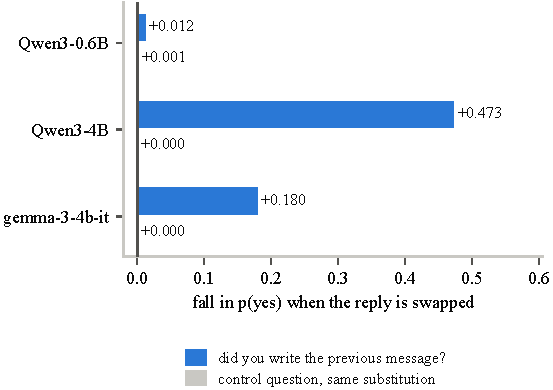
\includegraphics[width=0.5\figwidth]{figures/substitution}
\caption{Whether a subject notices that a reply in its own transcript is not
the one it wrote. The bar is how far its probability of answering \emph{yes}
falls when the reply is swapped for another of its own replies, paired by
prompt. The control question asks something unrelated to authorship under the
identical substitution, so a model that simply answers differently in an odd
transcript would move both bars. The appendix gives the underlying rates.}
\label{fig:substitution}
\end{figure}


\subsection{Can a subject tell its own reply from one it did not write?}

This asks whether a mind can tell, from its own transcript, that a message
attributed to it is not the one it produced. A stage swaps the subject's reply
for another reply the same model wrote to a different prompt, so style is held
fixed and only authorship changes. A fall on its own is not evidence, because a
strange transcript pushes a model around on any question, so the control is a
second question with nothing to do with authorship asked under the identical
substitution. Figure~\ref{fig:substitution} reports both. The control does not
move, and on the larger models the authorship question does. We therefore contend
that discriminating one's own output inside one's own context is a capability
some of these models have and others do not, and that it needs no judge.

\subsection{Does the architecture itself change how a mind talks about itself?}

Four compositions receive byte-identical prompts, and the grid is run twice: once
on prompts about the model and once on matched prompts about an ordinary topic,
so an architecture that changes every kind of answer equally cancels. The test
does not reject. We ran the grid again at three samples per cell and judged it
through a second model from a third family, regenerating none of the replies, and
the verdict did not move. The two judges agree on the conclusion and disagree on
the ranking, so the verdict belongs to the data while the cell that happens to
top it does not.
